\chapter{Implementation}

\section{Overview}
Building CAM-F from conception to deployment required integrating multiple computer vision technologies, real-time processing systems and some optimisation/reliability mechanisms. The implementation spans several interconnected components that work together to provide real-time continuity monitoring during active film production:

\textbf{Core Framework}: The monolithic backend provides a unified Python application managing all system operations. Built with FastAPI, it orchestrates frame capture, detector execution, and result aggregation. The system provides REST endpoints and Server-Sent Events for frontend communication. Only detector plugins execute in separate sandboxed processes.

\textbf{Detector Plugins}: Two proof-of-concept detectors demonstrate the framework's monitoring capabilities:
\begin{itemize}
\item \textbf{ClockDetector}: Combines YOLOv11 object detection with ResNet50-based time prediction model for analog clocks and PaddleOCR for digital displays.
\item \textbf{DifferenceDetector}: Implements co-attention networks for spatial change detection with specialised masking ignoring unnecessary motion anomalies.
\end{itemize}

\textbf{Production Optimisations}: To improve various performance metrics we implement error deduplication, multi-tier result caching with memory/disk persistence and failure recovery. We allow flexible control over the quality and resolution of an input along with capture rate. Monitoring using capture provides feed from various sources and for video upload we enable batch processing. Detectors are working in parallel with each other as frame pairs are pushed to their internal queues by the system.

On top of implementing a near deployment-ready application for script supervisors, we also incorporate a variety of small developer-friendly features that assist in research, building and debugging of new detectors. Although we aim for a high-quality final product, the main purpose of this implementation still remains within the scope of practical assessment and establishing a basic foundation for further research.

\section{Monitoring Pipeline}

\subsection{Capture to Storage}
The frame processing pipeline represents the core of CAM-F's operation. When monitoring begins, the capture service acquires frames from connected cameras or screen capture sources. Using OpenCV's platform-agnostic capture interface, the system supports multiple input sources: USB cameras, built-in webcams, DirectShow devices on Windows, V4L2 devices on Linux, screen and application capture. Regardless of source, frames arrive as NumPy arrays in BGR colour space, then undergo immediate serialisation to PNG format.

PNG's lossless compression preserves the visual fidelity while significantly decreasing file size. Instead of distributing BGR arrays to detectors and serialising them every time, we process and write it once. And then through file path communication we allow access to each PNG frame, which after the first read is cached by the OS. 

The storage service writes each frame to a hierarchical directory structure that mirrors production organisation. A frame captured during "Scene 4, Angle 2, Take 5" is located at a predictable path within the project file system: "data/storage/ProjectName\_1/Scene4\_2/Angle2\_3/Take5\_4/frames/frame\_000001.png". To maintain relationships with the database, while keeping customisation and readability, we utilise the ID-tagged naming convention \{Name\}\_\{DatabaseID\}.

\begin{figure}[h]
\centering
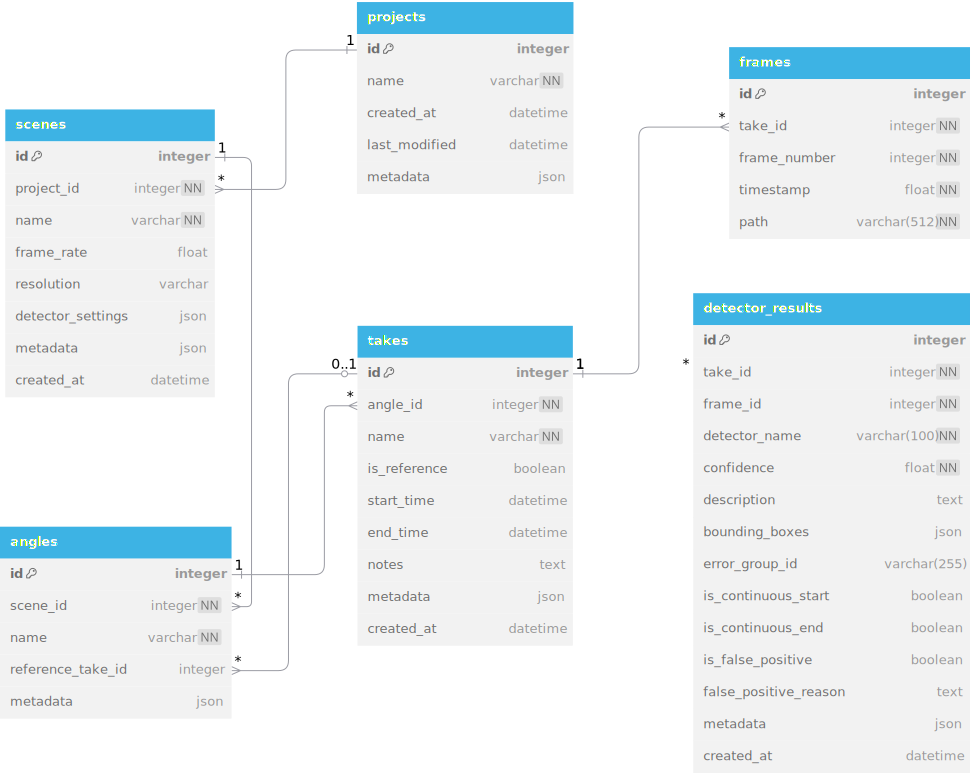
\includegraphics[width=0.9\textwidth]{figures/database.png}
\caption{Database schema showing relationships between projects, scenes, angles, takes, frames and detection results. The hierarchical structure enables efficient queries while foreign key constraints maintain referential integrity.}
\label{fig:database-relationships}
\end{figure}

\subsection{Reference Management}
Continuity detection fundamentally involves comparison. The goal is to identify what changed between the reference state and current state. The system automatically designates the first successful take of each scene angle as the reference baseline. This matches standard production practice where initial takes establish the continuity foundation, and the notes along with the images that the supervisor aggregates are used as reference.

We do not implement any sort of frame alignment or restrict specific timings to match total frame count for subsequent capture. While the frame rate is fixed for the entire scene configuration, due to the manual nature of capture controls, each take may still differentiatie by starting slightly earlier or being delayed. To mitigate the difference in frame counts, we stop processing at the lowest between the two. Depending on frame rate, temporal inconsistency in the action within the reference and current take has minor or no effect whatsoever on the detector and its accuracy. The implemented proof-of-concept detectors integrate the layer that deals with action interpretations.

At any point during principal photography, script supervisors may overwrite the reference take, of which each angle in a scene can only have one to avoid complexity. This change doesn't trigger the whole system overload, instead each take keeps the results from the latest processing session. However, at any point, the supervisor may redo the detection against a newly assigned reference. The system also allows user to select a specific take from any angle in the scene for a single instance processing.

\subsection{Frame Distribution}
Frame distribution to detectors employs a push-based model prioritising latency over throughput. When a new frame arrives, the framework immediately notifies all active detectors rather than waiting for detectors to pull for work. This design reflects production reality where immediate feedback during short reset windows proves more valuable than processing efficiency.

The distribution mechanism handles detector heterogeneity gracefully. Some detectors might opt to process frames individually, for example, a particular configuration of our ClockDetector examines current frames only. Others require frame pairs at all times. The framework abstracts these differences, providing each detector with appropriate frame sets based on their declared requirements in their manifest.

Queue management prevents system overload when detectors cannot maintain capture pace. Each detector receives an independent queue with configurable depth limits. When queues approach capacity, the framework begins selective frame dropping using importance-based prioritisation. First and last frames of each take receive highest priority as continuity errors frequently occur at shot boundaries. Middle frames are dropped first when processing falls behind.

\subsection{Result Aggregation}
Result aggregation begins immediately as detections arrive. The framework performs intelligent deduplication to reduce noise from persistent errors. Each detector's results are processed separately; when a detector identifies an anomaly, the system checks if it represents a continuation of the same one from previous frames. Spatial clustering uses two methods: bounding box overlap (IoU > 0.5) and center distance (<100 pixels) to determine if detections in consecutive frames represent the same underlying issue. This temporal-spatial grouping means a clock misalignment detected across multiple frames by a single detector appears as one continuous error rather than flooding supervisors with frame-by-frame alerts. However, to preserve unique findings and perspectives of each specialised detector the system deliberately maintains separation between them.

The bounding boxes, that describe the areas of concern within each frame, are stored as JSON metadata alongside the detection results. The system maintains complete data integrity - original frames remain untouched while detection overlays and annotations are stored separately in the database. On request these bounding boxes are generated as an overlay on top of the frames.

To assist research and development of new detectors we implement a small false positive management to handle cases where detectors are wrong. When supervisors identify a false positive, they can mark it directly in the interface with a reason. This allows for integration of supervised learning for specialised detectors. The reason for this integration was not just a mere gimmick for developers, it was important to allow script supervisors to have control over the results that they export. This way, they don't have to manually annotate exports with the wrong detections produced during monitoring.

The export system transforms aggregated results into production-ready documentation. PDF reports are generated with customisable notes from script supervisor, which can be edited within the UI, and a separate error section that provides a detailed frame-by-frame breakdown of all detections without duplications.

\section{ClockDetector}

\subsection{Detector Overview}
ClockDetector identifies temporal inconsistencies in film production by detecting and reading both analog and digital clocks. The implementation addresses two distinct challenges: interpreting analog clock faces with varying designs and perspectives, and recognising digital time displays across different device types. The detector employs separate processing pipelines for each clock type, unified through a common error reporting framework. When time discrepancies exceed configurable thresholds, the detector generates detailed continuity errors. 

\subsection{Analog Clocks}
Initial attempts to read analog clocks through geometric analysis showed undermining results. Direct calculation of hand angles failed to accommodate the diversity of clock designs, perspective distortions, and visual artifacts. When attempting to accurately detect the clock hands and calculate the displayed time, external visual factors significantly impacted performance, which led to very low accuracies below 40\%.

This limitation was clearly not practical for accurate real-time monitoring. After extensive literature review on time reading we decided to adopt the approach presented by Yang et al. in "It's About Time: Analog Clock Reading in the Wild" [23]. Their research demonstrates that analog clock reading benefits from a learning-based approach rather than geometric computation.

\begin{figure}[h]
\centering
\includegraphics[width=0.9\textwidth]{figures/ArchitectureClock.png}
\caption{ClockDetector processing pipeline. Input frame undergoes YOLOv11 localisation, followed by spatial transformation network (STN) for perspective normalisation, and finally ResNet50 classification to predict time as one of 720 discrete minute classes~\cite{yang2024}.}
\label{fig:clock-pipeline}
\end{figure}

\textbf{Detection Stage}: The implementation uses YOLOv11n for initial clock detection. This lightweight model identifies clock faces within frames, providing bounding boxes for subsequent processing. The nano variant balances detection accuracy with processing speed, achieving sub-200ms inference even on CPU hardware. We use a confidence threshold of 0.25. Even though this high tolerance level might trigger more false positives, those are filtered out at later stages of the pipeline.

\textbf{Time Reading Methodology}: Yang et al.'s approach treats time reading as a classification problem rather than a regression. Their model divides the 12-hour clock face into 720 discrete classes, representing each minute as a unique entity. The architecture employs two key components:
\begin{itemize}
\item \textbf{Spatial Transformer Network (STN)}: Learns to normalise clock appearance by predicting homography parameters. This module transforms oblique views into frontal perspectives, standardising clock orientation regardless of camera angle.
\item \textbf{ResNet50 Classifier}: Processes the aligned clock image to predict one of 720 time classes. The classifier benefits from the STN's normalisation, focusing on time determination rather than handling perspective variations.
\end{itemize}

\begin{figure}[h]
\centering
\includegraphics[width=0.9\textwidth]{figures/Clocks.png}
\caption{ClockDetector performance on challenging cases. Top row: Successful detections despite (a) partial occlusion, (b) extreme viewing angle, (c) motion blur. Bottom row: Failure cases due to (d) severe distortion, (e) ambiguous hand positions, (f) decorative clock design.}
\label{fig:clock-examples}
\end{figure}

Unlike the geometric analysis tested initially, this approach manages to accurately predict time even with some of the constraints: decorative or artistic clock faces with non-standard markers, partially occluded clock hands, variable hand designs (arrows, rectangles, ornate styles), shadows and reflections that confuse edge detection. The model's training on synthetic data with extensive augmentation enables generalisation to real-world clocks. Yang et al. report 80.4\% top-1 accuracy on COCO clock dataset.

\subsection{Digital Clocks}
Digital clock recognition presents a slightly different challenge than analog. Digital displays vary significantly in appearance from seven-segment LED displays to modern LCD screens. Each display type exhibits unique characteristics and varying contrast ratios.

\textbf{OCR Technologies}: Evaluation of available OCR solutions revealed significant performance differences for text detection. The seven-segment display study by Low et al. provides comprehensive analysis of OCR effectiveness on digital timepieces [24]. Their findings directly informed implementation choices for the detector.

Standard OCR tools like Tesseract and EasyOCR demonstrated poor performance on both regular text and seven-segment displays. Due to their limited training primarily on conventional fonts, they struggle to distinguish a high variety of digital clock faces. PaddleOCR, on the other hand, provided an optimal solution. Even though the study showed much higher scores of PARSeq's accuracy for seven-segment digits, PaddleOCR proved to be a good middle ground for performing text recognition of any kind.

\textbf{Processing Strategy}: Microwaves, smartphones, digital alarm clocks and watches, each presents time differently and in itself is a unique entity. Unfortunately, due to limitations of detection models like YOLO, attempting to localise the display and then perform OCR proved to be inaccurate. Missing simple alarm clock boxes or small seven-segment displays on other devices we had to opt for full OCR applied to the entire frame. This design trades computational efficiency for comprehensive coverage. The OCR engine examines all text-like regions, filtering results through time-pattern matching:

\begin{verbatim}
# Common time patterns (24-hour and 12-hour formats)
        self.time_patterns = [
            r'(\d{1,2}:\d{2}:\d{2})',                # Full time with seconds: 12:34:56
            r'(\d{1,2}:\d{2})',                      # Time without seconds: 12:34
            r'(\d{1,2}:\d{2}(?::\d{2})?\s*[APap][Mm])',  # 12-hour format: 12:34 PM
            r'(\d{1,2}[.:]\d{2}[.:]\d{2})',          # Alternative separators with seconds
            r'(\d{1,2}[.:]\d{2})',                   # Alternative separators without seconds
            r'(\d{1,2}\s*:\s*\d{2}\s*:\s*\d{2})',    # With spaces around colons
            r'(\d{1,2}\s*:\s*\d{2})',                # With spaces, no seconds
        ]
\end{verbatim}

\subsection{Validation and Error Reporting}
Reading individual timepieces is at the core of the detector, but we still need to add semantic value to the results and validate temporal continuity. The system maintains time progression records, comparing detected times from displays in either current or reference. 

For the sake of performance, if the script supervisor configures the detector for a specific time range, the detector would only request and process current frames instead of pairs. Since ground truth is now established through a given value, time detected in reference take is irrelevant. Otherwise, if no configuration for time range was provided, we utilise the first detected clock in the reference as ground truth for the scene's temporal validation. Clock detector identifies 3 main anomaly types:
\begin{itemize}
\item \textbf{Continuous flow}: Each subsequent clock after the first registered in the current frame should remain at a constant time or advance minimally.
\item \textbf{Time uniformity}: Every clock in a take should display near the same time.
\item \textbf{Narrative consistency}: The time of the scene should match across takes.
\end{itemize}

\section{DifferenceDetector}

\subsection{Detector Overview}
DifferenceDetector embodies a more conventional concept of automated continuity monitoring. It identifies visual changes between frame pairs that cannot be attributed to expected variations such as camera movement or actor motion. A similar idea was used in Pickup and Zisserman's 2009 study on film continuity where they computed pixel-wise differences between registered frames [5]. Unlike their pixel-based approach that flags every minor variation, this detector instead implements learned feature representations to distinguish meaningful changes from acceptable differences.

Traditional pixel-comparison would fail in production environment because it cannot differentiate between:
\begin{itemize}
\item A coffee mug that has genuinely moved (continuity error)
\item The same coffee mug appearing different due to lighting changes (acceptable variation)
\item A coffee mug at a slightly different angle due to camera movement (acceptable variation)
\end{itemize}

The detector was built upon the work completed by Sachdeva and Zisserman "The Change You Want to See" [22]. Their approach uses deep neural networks to extract high-level features from images at multiple spatial resolutions. These features capture object characteristics that remain consistent despite surface-level variations. When the model processes a coffee mug, it learns representations that are invariant to lighting changes and minor viewpoint shifts, enabling robust comparison between frames.

\subsection{Co-Attention Mechanism}
The architecture from Sachdeva and Zisserman employs co-attention mechanisms to establish implicit correspondences between frame pairs. This approach eliminates the need for explicit geometric registration, which often fails in real-world scenarios. Their architecture processes frame pairs through (see Figure 4.4):

\textbf{Feature Encoding}: A ResNet50 encoder extracts feature maps at three spatial resolutions from the last three blocks. These multi-scale representations capture both fine details and broader context.

\textbf{Co-Attention Module}: Each spatial location in one image's features attends to all locations in the other image's features. The attention mechanism computes:
\begin{itemize}
\item Query projections from the first image
\item Key projections from the second image
\item Attention weights through scaled dot-product
\item Weighted aggregation of features
\end{itemize}
The attended features are concatenated with the original features, providing both local information and cross-image context.

\textbf{Decoding}: A U-Net decoder with skip connections upsamples the conditioned features back to full resolution. Concurrent spatial and channel squeeze-and-excitation (scSE) blocks enhance feature representations.

\textbf{Detection}: A CenterNet head produces bounding box predictions for changed regions in both images simultaneously.

\begin{figure}[h]
\centering
\includegraphics[width=0.9\textwidth]{figures/ArchitectureDifference.png}
\caption{DifferenceDetector architecture based on co-attention networks. ResNet50 extracts multi-scale features, co-attention modules establish implicit correspondences, and CenterNet heads detect changes without explicit registration~\cite{sachdeva2023change}.}
\label{fig:difference-architecture}
\end{figure}

\subsection{Specialised Masking and Filtering}
During principal photography, takes may slightly differentiate, especially when it comes to actors' performance interpretation. While Sachdeva and Zisserman's model excels at detecting changes between a pair of frames, it has no semantic context of narrative and filming variations.

Inspired by Pickup and Zisserman's observation about masking moving objects in their continuity error detection work [5], we implement a pre-processing stage that removes regions containing humans and animals before applying the change detection model. We use Detectron2's Mask R-CNN to identify humans and animals in both frames. These detected regions are expanded by 10\% to account for motion blur and edge uncertainties, then filled with neutral grey (128, 128, 128) to prevent artificial edges. This preprocessing ensures the change detection model focuses only on static scene elements where continuity errors can occur, rather than being distracted by unnecessary motion.

Neural network outputs undergo multi-stage filtering to produce practical results. Initial confidence filtering removes detections below 0.10. Subsequently, we filter by area (minimum 0.01\% of frame) and aspect ratio (0.1-10.0), eliminating sensor noise while preserving small significant changes. Finally, creature filtering suppresses detections with >30\% overlap with masked regions, accommodating partial occlusions while preventing false positives from motion.

\begin{figure}[h]
\centering
\includegraphics[width=0.9\textwidth]{figures/difference pipeline.png}
\caption{DifferenceDetector processing pipeline. (a) Reference and current frames. (b) Person segmentation masks (dilated for safety). (c) Co-attention difference map highlighting changes. (d) Final detections after filtering, showing moved prop (red box) while ignoring actor position changes.}
\label{fig:difference-pipeline}
\end{figure}

\subsection{Validation and Error Reporting}
Due to the already heavy computational complexity of the core implementation, we decided to opt for a streamlined error reporting approach. DifferenceDetector uses a unified "visual\_change" error type for all detections, avoiding the computational overhead of semantic classification to maintain real-time performance. Instead of categorising changes into types like "cup misplacement" or "missing remote", the system simply provides spatial data along with confidence scores. By focusing on accurate detection rather than interpretation, the detector delegates assessment to continuity professionals, where they can apply their expertise efficiently.

\section{Additional Features} 

\subsection{Parallel Processing}
Early prototyping showed that a universal detector would introduce enormous complexity and high performance overhead. Combining multiple technologies into one-for-all continuity monitoring process wouldn't be feasible. This constraint shaped the modular architecture, where specialised detectors operate in parallel to maintain real-time performance.

As previously discussed, each detector maintains its own PriorityQueueManager handling frame distribution. The framework spawns detector processes once a take is opened. It allows us to initialise detectors while the user prepares a new monitoring session. Once the capture starts we push frames to each detector's queue as they come. Non-blocking queues enable asynchronous processing: ClockDetector might analyse frame 10 whilst DifferenceDetector processes frame 7. Detection results are sent immediately back to the database and are rendered both as bounding boxes on the frame display and an alert in the detected anomalies table. Configurable queue limits prevent memory exhaustion without throttling faster detectors, ensuring consistent throughput regardless of individual detector complexity.

\subsection{Error Deduplication}
Production testing revealed that a single persistent error could generate hundreds of redundant alerts across multiple frames. The implementation employs two deduplication stages: real-time processing during capture and post-processing for batch analysis.

Real-time deduplication tracks errors across consecutive frames using spatial matching criteria. The system considers errors as matching when either their bounding boxes overlap by more than 50\%, IoU (Intersection over Union) > 0.5, or their centre points lie within 100 pixels of each other. Additionally, errors must originate from the same detector and contain matching description text. The algorithm requires errors to appear in consecutive frames to maintain continuity chains, marking them as inactive after a 5-frame absence. The database tracks continuous groups by storing first and last frame references. 

\subsection{Video Uploads}
During the development of the framework and detectors, assessment of the full workflow proved to have significant overhead: connecting capture devices, attempting to imitate specific anomalies and doing that repeatedly to mirror real production workflows. Implementing video upload proved to be a valuable addition to the rest of features to enhance both developers' and script supervisors' experiences. 

Upload uses OpenCV's \texttt{VideoCapture} to extract frames from video files at a configurable sample rate. The system loads the video file, calculates the sampling interval based on the scene's target frame rate versus the video's native frame rate, then iterates through frames saving them as individual PNG files with lossless compression (level 3) via the storage service, which is consistent with the live capture. With \texttt{BatchProcessor} videos are handled in parallel segments using Python's \texttt{ThreadPoolExecutor} to increase upload speed.